\documentclass[12pt,]{krantz}
\usepackage{lmodern}
\usepackage{amssymb,amsmath}
\usepackage{ifxetex,ifluatex}
\usepackage{fixltx2e} % provides \textsubscript
\ifnum 0\ifxetex 1\fi\ifluatex 1\fi=0 % if pdftex
  \usepackage[T1]{fontenc}
  \usepackage[utf8]{inputenc}
\else % if luatex or xelatex
  \ifxetex
    \usepackage{mathspec}
  \else
    \usepackage{fontspec}
  \fi
  \defaultfontfeatures{Ligatures=TeX,Scale=MatchLowercase}
\fi
% use upquote if available, for straight quotes in verbatim environments
\IfFileExists{upquote.sty}{\usepackage{upquote}}{}
% use microtype if available
\IfFileExists{microtype.sty}{%
\usepackage{microtype}
\UseMicrotypeSet[protrusion]{basicmath} % disable protrusion for tt fonts
}{}
\usepackage[margin=1in]{geometry}
\usepackage{hyperref}
\PassOptionsToPackage{usenames,dvipsnames}{color} % color is loaded by hyperref
\hypersetup{unicode=true,
            pdftitle={EDISON 사이언스 앱을 사용한 비구획분석과 생물학적동등성 분석의 통합},
            colorlinks=true,
            linkcolor=Maroon,
            citecolor=Blue,
            urlcolor=Blue,
            breaklinks=true}
\urlstyle{same}  % don't use monospace font for urls
\usepackage{color}
\usepackage{fancyvrb}
\newcommand{\VerbBar}{|}
\newcommand{\VERB}{\Verb[commandchars=\\\{\}]}
\DefineVerbatimEnvironment{Highlighting}{Verbatim}{commandchars=\\\{\}}
% Add ',fontsize=\small' for more characters per line
\usepackage{framed}
\definecolor{shadecolor}{RGB}{248,248,248}
\newenvironment{Shaded}{\begin{snugshade}}{\end{snugshade}}
\newcommand{\AlertTok}[1]{\textcolor[rgb]{0.94,0.16,0.16}{#1}}
\newcommand{\AnnotationTok}[1]{\textcolor[rgb]{0.56,0.35,0.01}{\textbf{\textit{#1}}}}
\newcommand{\AttributeTok}[1]{\textcolor[rgb]{0.77,0.63,0.00}{#1}}
\newcommand{\BaseNTok}[1]{\textcolor[rgb]{0.00,0.00,0.81}{#1}}
\newcommand{\BuiltInTok}[1]{#1}
\newcommand{\CharTok}[1]{\textcolor[rgb]{0.31,0.60,0.02}{#1}}
\newcommand{\CommentTok}[1]{\textcolor[rgb]{0.56,0.35,0.01}{\textit{#1}}}
\newcommand{\CommentVarTok}[1]{\textcolor[rgb]{0.56,0.35,0.01}{\textbf{\textit{#1}}}}
\newcommand{\ConstantTok}[1]{\textcolor[rgb]{0.00,0.00,0.00}{#1}}
\newcommand{\ControlFlowTok}[1]{\textcolor[rgb]{0.13,0.29,0.53}{\textbf{#1}}}
\newcommand{\DataTypeTok}[1]{\textcolor[rgb]{0.13,0.29,0.53}{#1}}
\newcommand{\DecValTok}[1]{\textcolor[rgb]{0.00,0.00,0.81}{#1}}
\newcommand{\DocumentationTok}[1]{\textcolor[rgb]{0.56,0.35,0.01}{\textbf{\textit{#1}}}}
\newcommand{\ErrorTok}[1]{\textcolor[rgb]{0.64,0.00,0.00}{\textbf{#1}}}
\newcommand{\ExtensionTok}[1]{#1}
\newcommand{\FloatTok}[1]{\textcolor[rgb]{0.00,0.00,0.81}{#1}}
\newcommand{\FunctionTok}[1]{\textcolor[rgb]{0.00,0.00,0.00}{#1}}
\newcommand{\ImportTok}[1]{#1}
\newcommand{\InformationTok}[1]{\textcolor[rgb]{0.56,0.35,0.01}{\textbf{\textit{#1}}}}
\newcommand{\KeywordTok}[1]{\textcolor[rgb]{0.13,0.29,0.53}{\textbf{#1}}}
\newcommand{\NormalTok}[1]{#1}
\newcommand{\OperatorTok}[1]{\textcolor[rgb]{0.81,0.36,0.00}{\textbf{#1}}}
\newcommand{\OtherTok}[1]{\textcolor[rgb]{0.56,0.35,0.01}{#1}}
\newcommand{\PreprocessorTok}[1]{\textcolor[rgb]{0.56,0.35,0.01}{\textit{#1}}}
\newcommand{\RegionMarkerTok}[1]{#1}
\newcommand{\SpecialCharTok}[1]{\textcolor[rgb]{0.00,0.00,0.00}{#1}}
\newcommand{\SpecialStringTok}[1]{\textcolor[rgb]{0.31,0.60,0.02}{#1}}
\newcommand{\StringTok}[1]{\textcolor[rgb]{0.31,0.60,0.02}{#1}}
\newcommand{\VariableTok}[1]{\textcolor[rgb]{0.00,0.00,0.00}{#1}}
\newcommand{\VerbatimStringTok}[1]{\textcolor[rgb]{0.31,0.60,0.02}{#1}}
\newcommand{\WarningTok}[1]{\textcolor[rgb]{0.56,0.35,0.01}{\textbf{\textit{#1}}}}
\usepackage{longtable,booktabs}
\usepackage{graphicx,grffile}
\makeatletter
\def\maxwidth{\ifdim\Gin@nat@width>\linewidth\linewidth\else\Gin@nat@width\fi}
\def\maxheight{\ifdim\Gin@nat@height>\textheight\textheight\else\Gin@nat@height\fi}
\makeatother
% Scale images if necessary, so that they will not overflow the page
% margins by default, and it is still possible to overwrite the defaults
% using explicit options in \includegraphics[width, height, ...]{}
\setkeys{Gin}{width=\maxwidth,height=\maxheight,keepaspectratio}
\IfFileExists{parskip.sty}{%
\usepackage{parskip}
}{% else
\setlength{\parindent}{0pt}
\setlength{\parskip}{6pt plus 2pt minus 1pt}
}
\setlength{\emergencystretch}{3em}  % prevent overfull lines
\providecommand{\tightlist}{%
  \setlength{\itemsep}{0pt}\setlength{\parskip}{0pt}}
\setcounter{secnumdepth}{5}
% Redefines (sub)paragraphs to behave more like sections
\ifx\paragraph\undefined\else
\let\oldparagraph\paragraph
\renewcommand{\paragraph}[1]{\oldparagraph{#1}\mbox{}}
\fi
\ifx\subparagraph\undefined\else
\let\oldsubparagraph\subparagraph
\renewcommand{\subparagraph}[1]{\oldsubparagraph{#1}\mbox{}}
\fi

%%% Use protect on footnotes to avoid problems with footnotes in titles
\let\rmarkdownfootnote\footnote%
\def\footnote{\protect\rmarkdownfootnote}

%%% Change title format to be more compact
\usepackage{titling}

% Create subtitle command for use in maketitle
\newcommand{\subtitle}[1]{
  \posttitle{
    \begin{center}\large#1\end{center}
    }
}

\setlength{\droptitle}{-2em}

  \title{EDISON 사이언스 앱을 사용한 비구획분석과 생물학적동등성 분석의 통합}
    \pretitle{\vspace{\droptitle}\centering\huge}
  \posttitle{\par}
    \author{}
    \preauthor{}\postauthor{}
      \predate{\centering\large\emph}
  \postdate{\par}
    \date{2019-01-28}

\usepackage{kotex}

\begin{document}
\maketitle

{
\hypersetup{linkcolor=black}
\setcounter{tocdepth}{2}
\tableofcontents
}
\hypertarget{section}{%
\chapter*{책 머리에}\label{section}}



\includegraphics{logo-BE.jpg}

생물학적동등성은 비구획분석으로 계산된 약동학적 파라미터를 사용하여 통계 분석을 수행함으로 판단할 수 있다. 현재는 이러한 분석을 위해서 여러 상용 소프트웨어를 필요로 하는 복잡한 단계를 거쳐야 한다. 따라서 분석 시간이 오래 걸리고 많은 비용이 소모되었다. 본 저자들은 EDISON 사이언스 앱을 사용하여 이 두 과정을 통합하였고, 이로서 농도-시간 자료로부터 비구획분석과 생물학적동등성 통계 분석까지 연속적으로 가능하게 되었다. 본 연구가 제시하는 EDISON 사이언스 앱을 통한 방법을 통해 정확한 분석을 빠른 시간에 수행할 수 있을 뿐만 아니라 오류를 줄이고 비용을 절감하는 효과를 가져올 수 있다.

한성필†, 윤석규, 조용순, 김형섭, 배균섭*\\
서울아산병원 임상약리학과, 울산대학교병원, 서울특별시 송파구 올림픽로 43 길 88\\
E-mail: 한성필 \href{mailto:shan@acp.kr}{\nolinkurl{shan@acp.kr}} , 배균섭 \href{mailto:ksbae@acp.kr}{\nolinkurl{ksbae@acp.kr}}

\hypertarget{intro}{%
\chapter{서론}\label{intro}}

생물학적동등성시험(bioequivalence test)는 기존 의약품의 특허가 만료된 후, 해당 의약품을 동일하게 개발하여 판매하고자 할 때 수행하는 임상시험이다. {[}1{]} 기존 오리지날 의약품(Reference)과 새로 개발한 의약품 즉 시험약(Test)을 교차연구(crossover study)의 형태로 투여한 뒤, 혈중 농도로부터 구한 약동학적 파라미터(pharmacokinetic parameter) 를 비교하여 평가하게 된다. 비교평가항목은 검체가 혈액인 경우, 1회 투약 시 AUCt, Cmax, 반복투약 시 AUCτ, Css,max를 주로 사용한다. 다만, 니트로글리세린 설하정과 같이 빠른 약효를 나타내는 제제 등은 Tmax를 비교평가항목으로 추가하기도 한다.

약동학 파라미터는 로그정규분포(log-normal distribution)을 따르고, 대조약과 시험약의 산출된 곡선하 면적(AUC)과 최대 농도 Cmax의 geometric mean ratio가 0.8 \textasciitilde{} 1.25 이내일 때, 약동학적으로 동등하다고 평가하게 된다. {[}2{]}

생물학적 동등성을 평가하는데 통계학은 핵심적인 역할을 수행하고 있고, 통계적 분석을 위해서는 컴퓨터 소프트웨어가 필요하다. SAS, SPSS 등과 같은 통계처리 프로그램을 혹은 독자 개발된 프로그램으로 통계적 검정을 실시할 수 있다. {[}3{]}

그러나 각각의 소프트웨어가 사용하기 어렵고 과정이 복잡하며 큰 비용이 소모되었다. 특히 약동학 분석 초보자나 통계학 비전공자가 사용하기 어려웠다. 본 저자들은 EDISON 사이언스 앱을 사용하여 이 과정을 연속성을 지닌 한 과정으로 통합하였다. 본 연구가 제시하는 방법을 통해 쉽고 정확하고 비용이 들지 않는 빠른 비구획분석과 생물학적 동등성 분석이 가능하다는 것을 보이고자 한다.

\hypertarget{method}{%
\chapter{이론 및 계산방법}\label{method}}

\hypertarget{edison---r-}{%
\section{EDISON 사이언스 앱과 R 패키지}\label{edison---r-}}

본 분석에서 사용될 EDISON 사이언스 앱은 NonCompartEdison, edisonBE 두 종류이다. 각각 비구획분석과 생물학적동등성 통계 분석을 하게 되며 R 기반 {[}4{]} 으로 프로그래밍 되어 있다. 각각은 NonCompart와 BE라는 이름의 R 패키지 형태로 공개되어 배포 되고 있다. R 콘솔에서는 다음을 입력함으로서 각 라이브러리를 불러올 수 있다.

\begin{Shaded}
\begin{Highlighting}[]
\KeywordTok{install.packages}\NormalTok{(}\StringTok{"NonCompart"}\NormalTok{)}
\KeywordTok{install.packages}\NormalTok{(}\StringTok{"BE"}\NormalTok{)}

\KeywordTok{library}\NormalTok{(NonCompart)}
\KeywordTok{library}\NormalTok{(BE)}
\end{Highlighting}
\end{Shaded}

EDISON 사이언스 앱을 제작하는데 사용한 R 코드 및 자료(datasets)는 \url{https://github.com/asancpt/edison-noncompart}, \url{https://github.com/asancpt/edison-BE} 에 각각 공개되어 있다.

\hypertarget{section-1}{%
\section{모형}\label{section-1}}

\[
Y_{ijk} = \mu + S_{ik} + P_{j} + F_{j,k} + C_{(j-1,k)} + \varepsilon_{ijk}
\]

이때에 μ; 전체 평균, Sik; k 번째 sequence에서 i 번째 subject의 효과(랜덤), Pj : j번째 period 의 효과(고정), Fj, k; k 번째 sequence에서 j 번째 period의 제제의 효과(고정), C(j-1,k): k 번째 sequence에서(j-1) 번째 period의 잔류효과(고정), εijk : 오차항으로 정의한다. 이 모델에서 사용하는 가정은 1) Sik ∼ N(0,σs²), 2) εijk ∼ N(0,σe²), 3) Sik 와 εijk가 독립이라는 세가지 이다. 이때 (μT - μR)에 대한 (1-2α)×100\% 신뢰구간이 ln(0.8), ln(1.25) 안에 들어가면 두제제가 생물학적으로 동등하다 결론을 내릴 수 있다.

\hypertarget{sas-}{%
\section{SAS 코드}\label{sas-}}

SAS는 통계 패키지중에서는 가장 방대하고 다양한 분석을 제공하고 전 세계적으로 생물학적동등성의 판단을 위해 표준으로 사용되고 있다. 다음과 같이 2x2 교차설계 자료를 분석하기 위한 SAS 코드 (PROC GLM, PROC MIXED, SAS version 9.4)를 작성하고 EDISON 사이언스 앱에서 계산된 결과와 비교하였다.

\begin{verbatim}
PROC GLM DATA=BE OUTSTAT=STATRES; /* GLM use only complete subjects. */
CLASS SEQ PRD TRT SUBJ;
MODEL LNAUCL = SEQ SUBJ(SEQ) PRD TRT;
RANDOM SUBJ(SEQ)/TEST;
LSMEANS TRT /PDIFF=CONTROL('R') CL ALPHA=0.1 COV OUT=LSOUT;

PROC MIXED DATA=BE; /* MIXED uses all data. */
CLASS SEQ TRT SUBJ PRD;
MODEL LNAUCL = SEQ PRD TRT;
RANDOM SUBJ(SEQ);
ESTIMATE 'T VS R' TRT -1 1 /CL ALPHA=0.1;
ODS OUTPUT ESTIMATES=ESTIM COVPARMS=COVPAR;
\end{verbatim}

\hypertarget{section-2}{%
\section{자료의 형태, 자료의 구성요소}\label{section-2}}

2x2 cross-over design이 가장 기본적인 디자인(통상 RT / TR)으로 사용된다. 피험자를 무작위로 두 군으로 나누어 각 군별로 동일 성분의 대조약과 시험약을 각각 투여(제1기 투약)하고 피험자별로 투약 전후 정해진 시간마다 채혈하고 농도 측정한다. 이전에 투여한 약이 모두 배설될 정도로 충분한 기간 경과 (보통 반감기의 5배 이상) 후 각 군별로 대조약과 시험약을 바꾸어 각각 투여하고(제2기 투약) 동일하게 혈액 채취 및 혈중농도 측정하게 된다.
본 논문에서는 위와 같은 시나리오로 시뮬레이션을 통해 얻어진 약동학 파라미터를 사용해 자료가 구성되었고, EDISON 사이언스 앱인 NonCompartEdison에서 입력으로 사용될 자료의 형태는 Table 1와 같다. SEQ (sequence), TRT (treatment), SUBJ (subject), and PRD (period, 기)의 자료가 열 형태로 제시되어야 하며 이는 edisonBE 앱에서 사용되는 약동학 파라미터 자료에도 일종의 primary key로 사용되기 때문에 유사한 형태로 보존되어야 한다. 33명의 대상자의 개인별 농도-시간 그래프는 Figure 1에 나타내었다.

\hypertarget{result}{%
\chapter{결과}\label{result}}

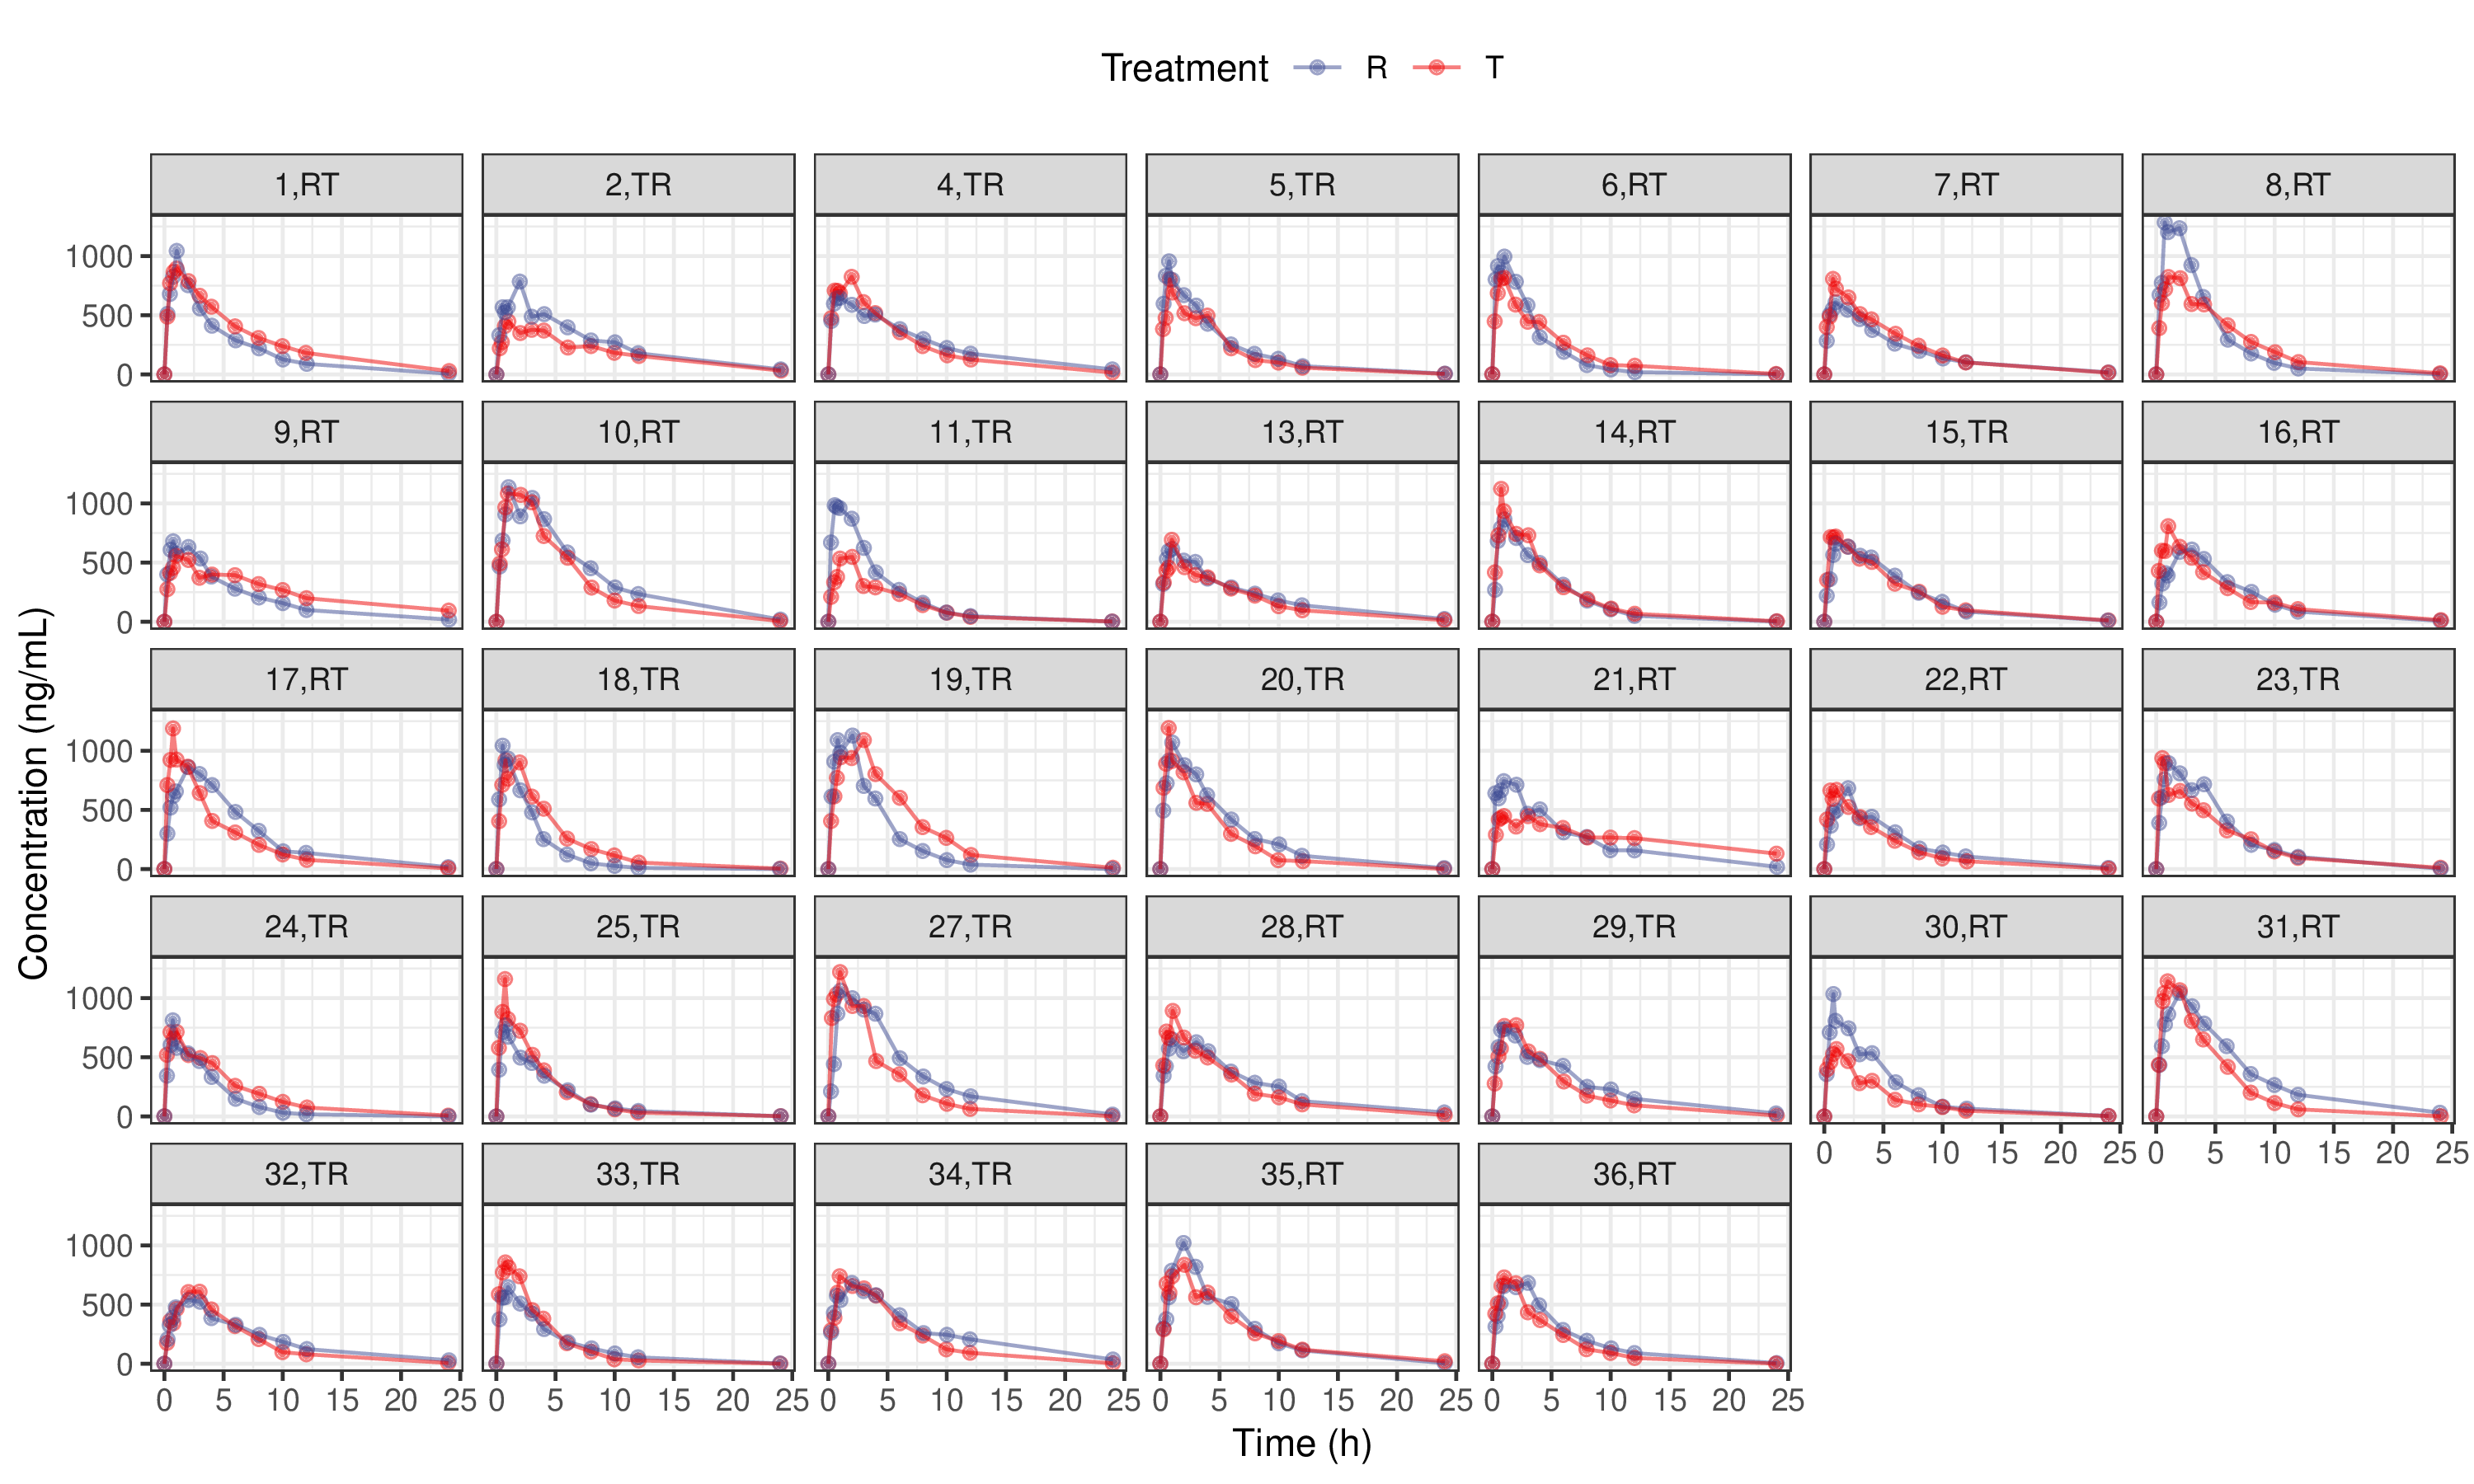
\includegraphics{assets-paper/figure-1.png}

Figure 1. Concentration-time curves of raw data (N=33)

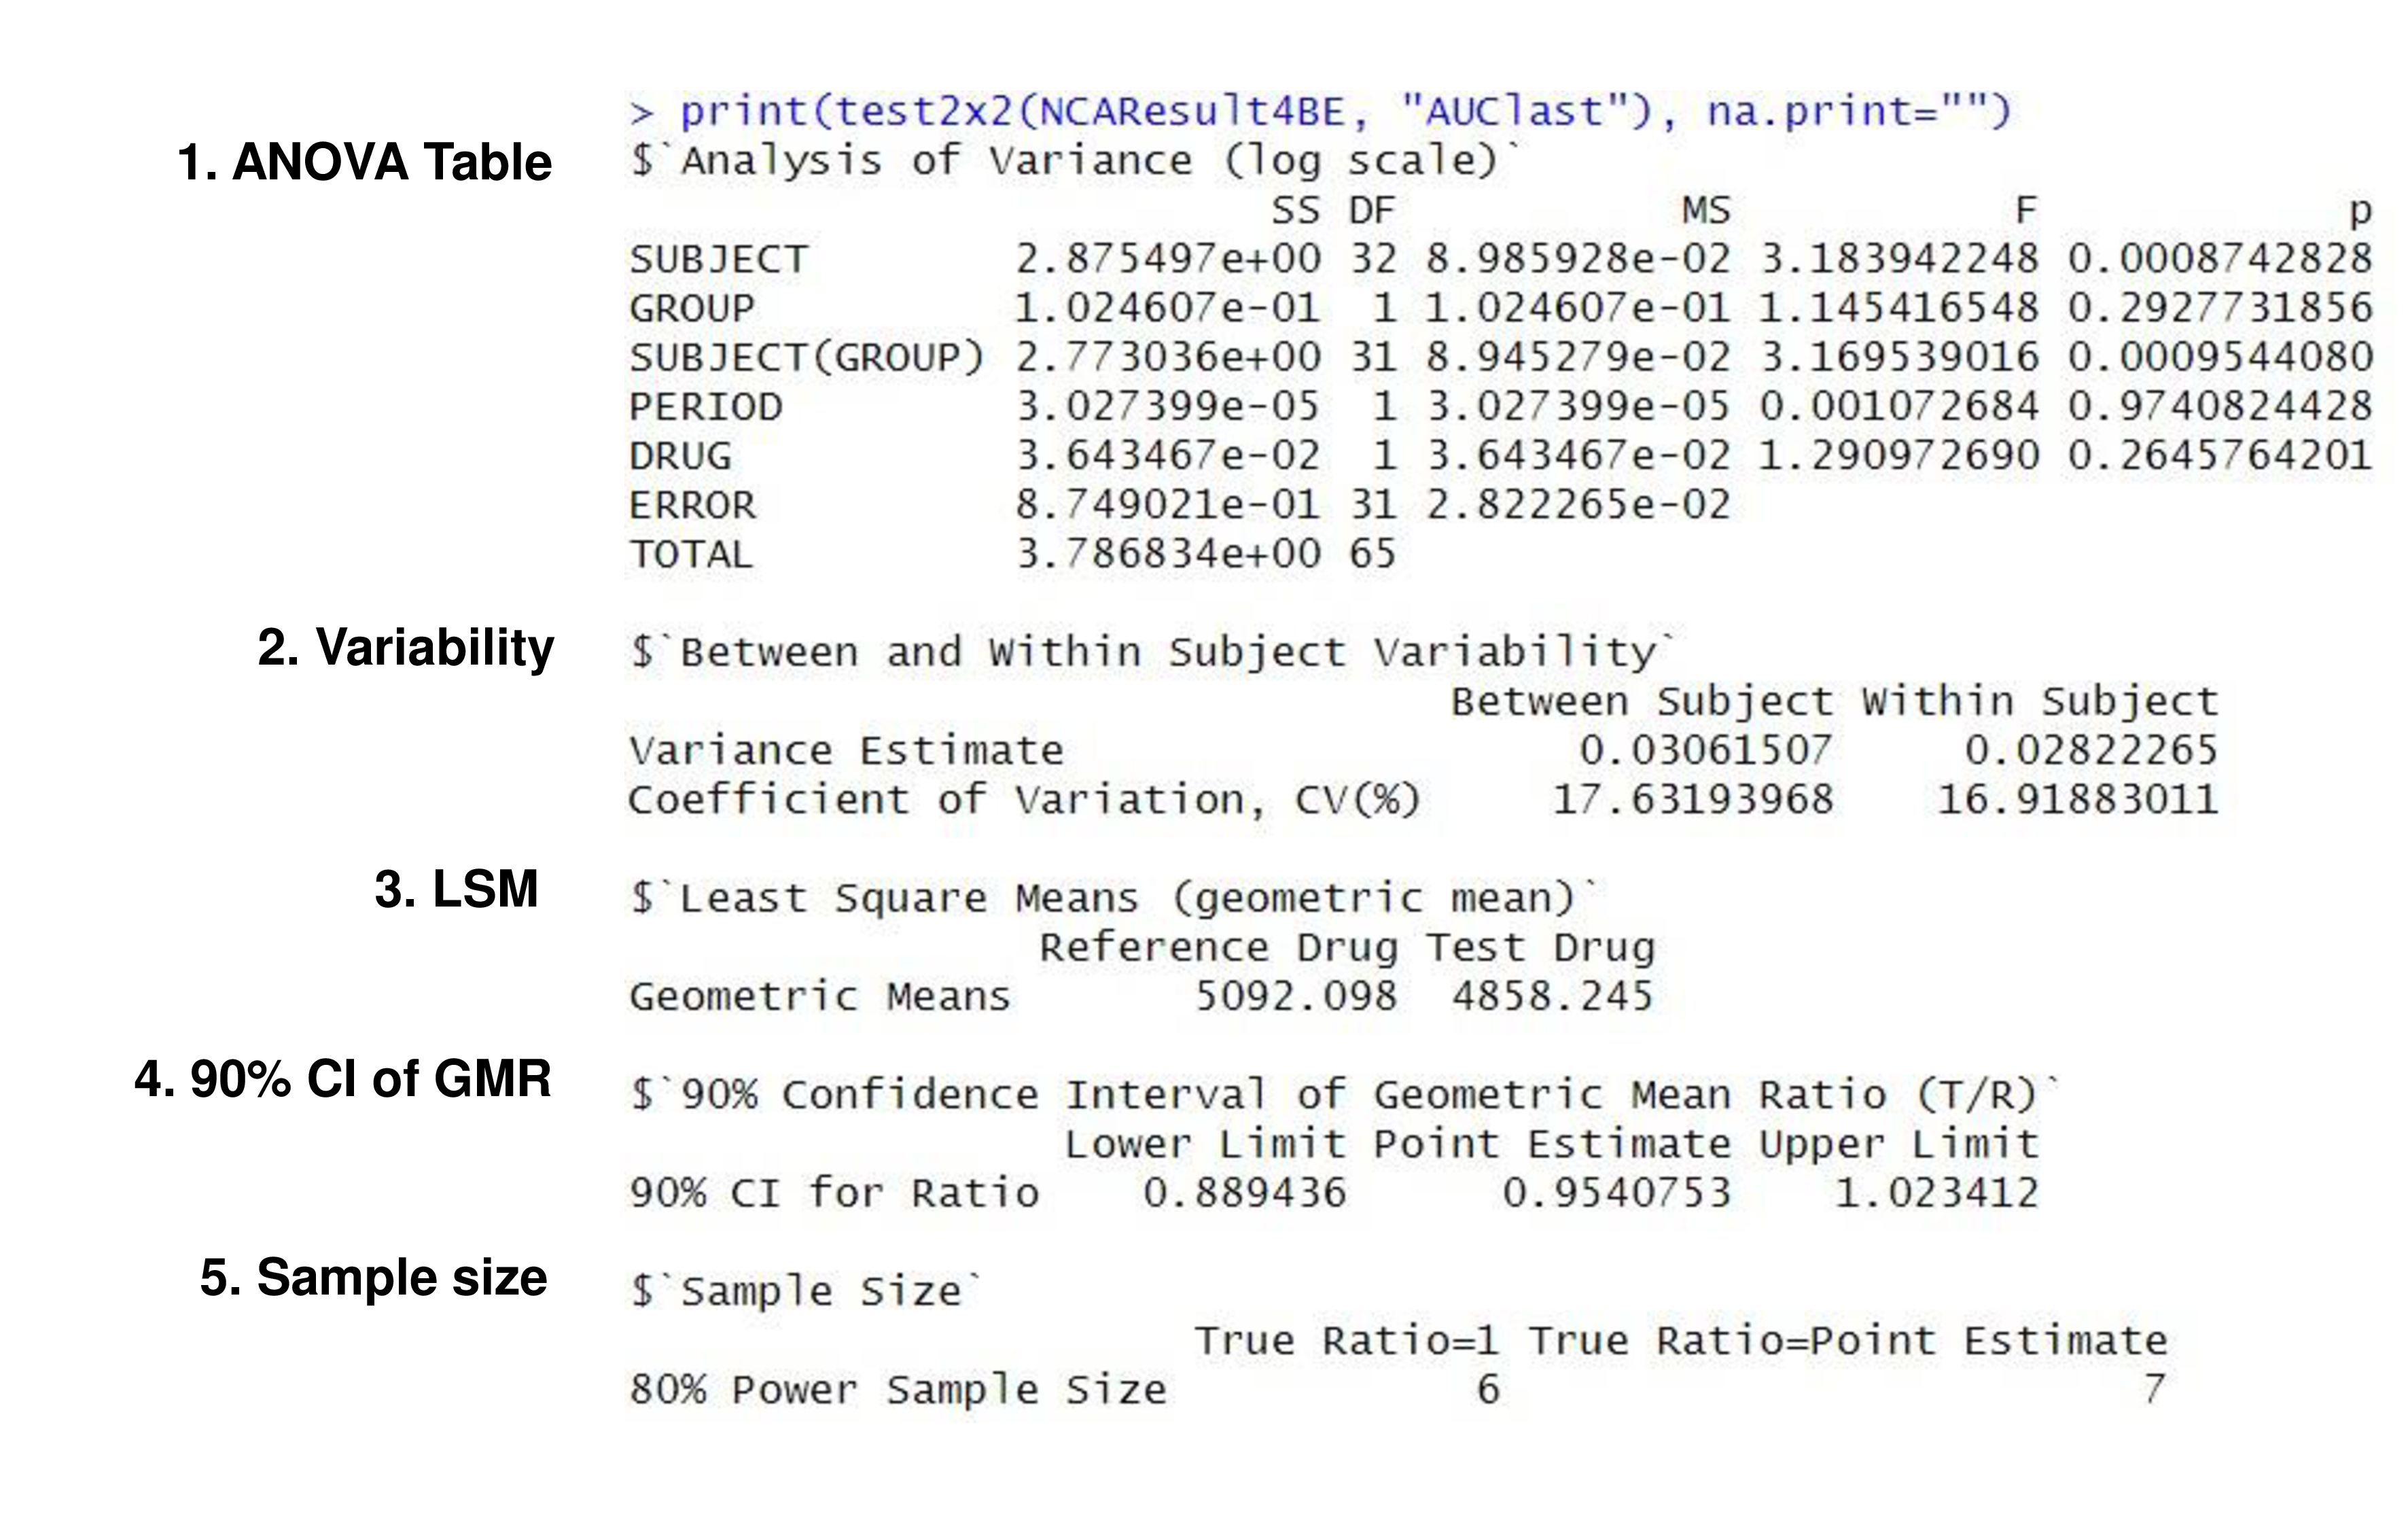
\includegraphics{assets-paper/figure-2.png}

Figure 2. Output format of bioequivalence tests performed by BE R package.

\hypertarget{noncompartedison---}{%
\section{NonCompartEdison 앱을 통한 비구획분석}\label{noncompartedison---}}

농도-시간 입력 자료(Table 1)는 NonCompartEdison 앱을 통해서 처리되어 약동학 파라미터가 계산되어 표형태의 출력 자료가 된다. (Table 2) 이것이 다시 edisonBE 앱의 입력자료가 되어 생물학적동등성 분석을 위해 쓰이게 된다.

\hypertarget{edisonbe----}{%
\section{edisonBE 앱을 통한 생물학적동등성 판단}\label{edisonbe----}}

약동학 파라미터가 입력 자료가 되어 edisonBE 앱을 통해 처리되고 생물학적동등성 판단을 위한 ANOVA 표, 변이 (variability), Least square mean (LSM), geometric mean ratio (GMR)의 90\% 신뢰구간, 샘플 수의 계산이 수행된다. (Figure 2) 본 자료로 계산한 AUClast는 생물학적 동등성 기준을 만족하고 있다.

\hypertarget{sas--}{%
\section{90\% 신뢰구간의 SAS 결과값과 비교}\label{sas--}}

위 과정으로 얻어진 계산값은 가장 정확하게 생물학적 동등성을 평가하고 있어 표준으로 사용되는SAS 소프트웨어 결과값과 완전히 동일하였다. (Table 3)

\hypertarget{section-3}{%
\section{샘플 수 계산}\label{section-3}}

BE 패키지를 통한 분석은 Between subject CV값과 Within Subject CV를 계산한다. 이에 근거하여 80\%의 파워로 계산한 샘플수 계산을 수행하며 T/R 비 (ratio) 가 1일 때와 점추정치일 경우를 각각 계산하여 결과를 출력한다.
본 자료로 계산한 AUClast의 개인간 (between subject) CV값은 17.63\%, 개인내 (within subject) CV값은 16.92\%인 것을 알 수 있고 80\% 파워로 계산한 샘플 수는 GMR이 1인 경우 6명, 점추정치인 0.95와 같은 경우 7명이 나오게 된다. (Figure 2)

Table 1. An example of the raw concentration-time data used for EDISON Science Apps. The dataset was simulated based on the 2x2 crossover design.

\begin{verbatim}
SUBJ    GRP PRD TRT nTIME   TIME    CONC
1   RT  1   R   0   0   0
1   RT  1   R   0.25    0.26    511.3
1   RT  1   R   0.5 0.46    678.79
1   RT  1   R   …   …   …
1   RT  2   T   0   0   0
1   RT  2   T   0.25    0.25    487.62
1   RT  2   T   0.5 0.48    769.6
…   …   …   …   …   …   …
5   TR  1   T   0   0   0
5   TR  1   T   0.25    0.23    382.79
5   TR  1   T   0.5 0.45    477.03
5   TR  1   T   …   …   …
5   TR  2   R   0   0   0
5   TR  2   R   0.25    0.28    596.98
5   TR  2   R   0.5 0.47    832.76
5   TR  2   R   …   …   …
…   …   …   …   …   …   …
\end{verbatim}

Table 2. The raw pharmacokinetic data calculated by NonCompartEdison App

\begin{verbatim}
SUBJ    GRP PRD TRT AUClast Cmax    Tmax
1   RT  1   R   5018.927    1043.13 1.04
1   RT  2   T   6737.507    894.21  1.03
2   TR  1   T   4373.97 447.26  1.01
2   TR  2   R   6164.276    783.92  1.98
4   TR  1   T   5592.993    824.42  1.97
4   TR  2   R   5958.16 646.31  0.97
5   TR  1   T   3902.59 803.7   0.8
5   TR  2   R   4620.156    955.3   0.74
\end{verbatim}

Table 3. Comparison of 90\% confidence interval for the ratio of the geometric means of (A) AUClast and (B) Cmax

\begin{verbatim}
(A)
Analysis    Lower Limit Point Estimate  Upper Limit
EDISON Science App  0.88944 0.95408 1.02341
SAS: PROC GLM   0.88944 0.95408 1.02341
SAS: PROC MIXED 0.88944 0.95408 1.02341

(B)         
Analysis    Lower Limit Point Estimate  Upper Limit
EDISON Science App  0.90136 0.97984 1.06515
SAS: PROC GLM   0.90136 0.97984 1.06515
SAS: PROC MIXED 0.90136 0.97984 1.06515
\end{verbatim}

\hypertarget{discussion}{%
\chapter{논의}\label{discussion}}

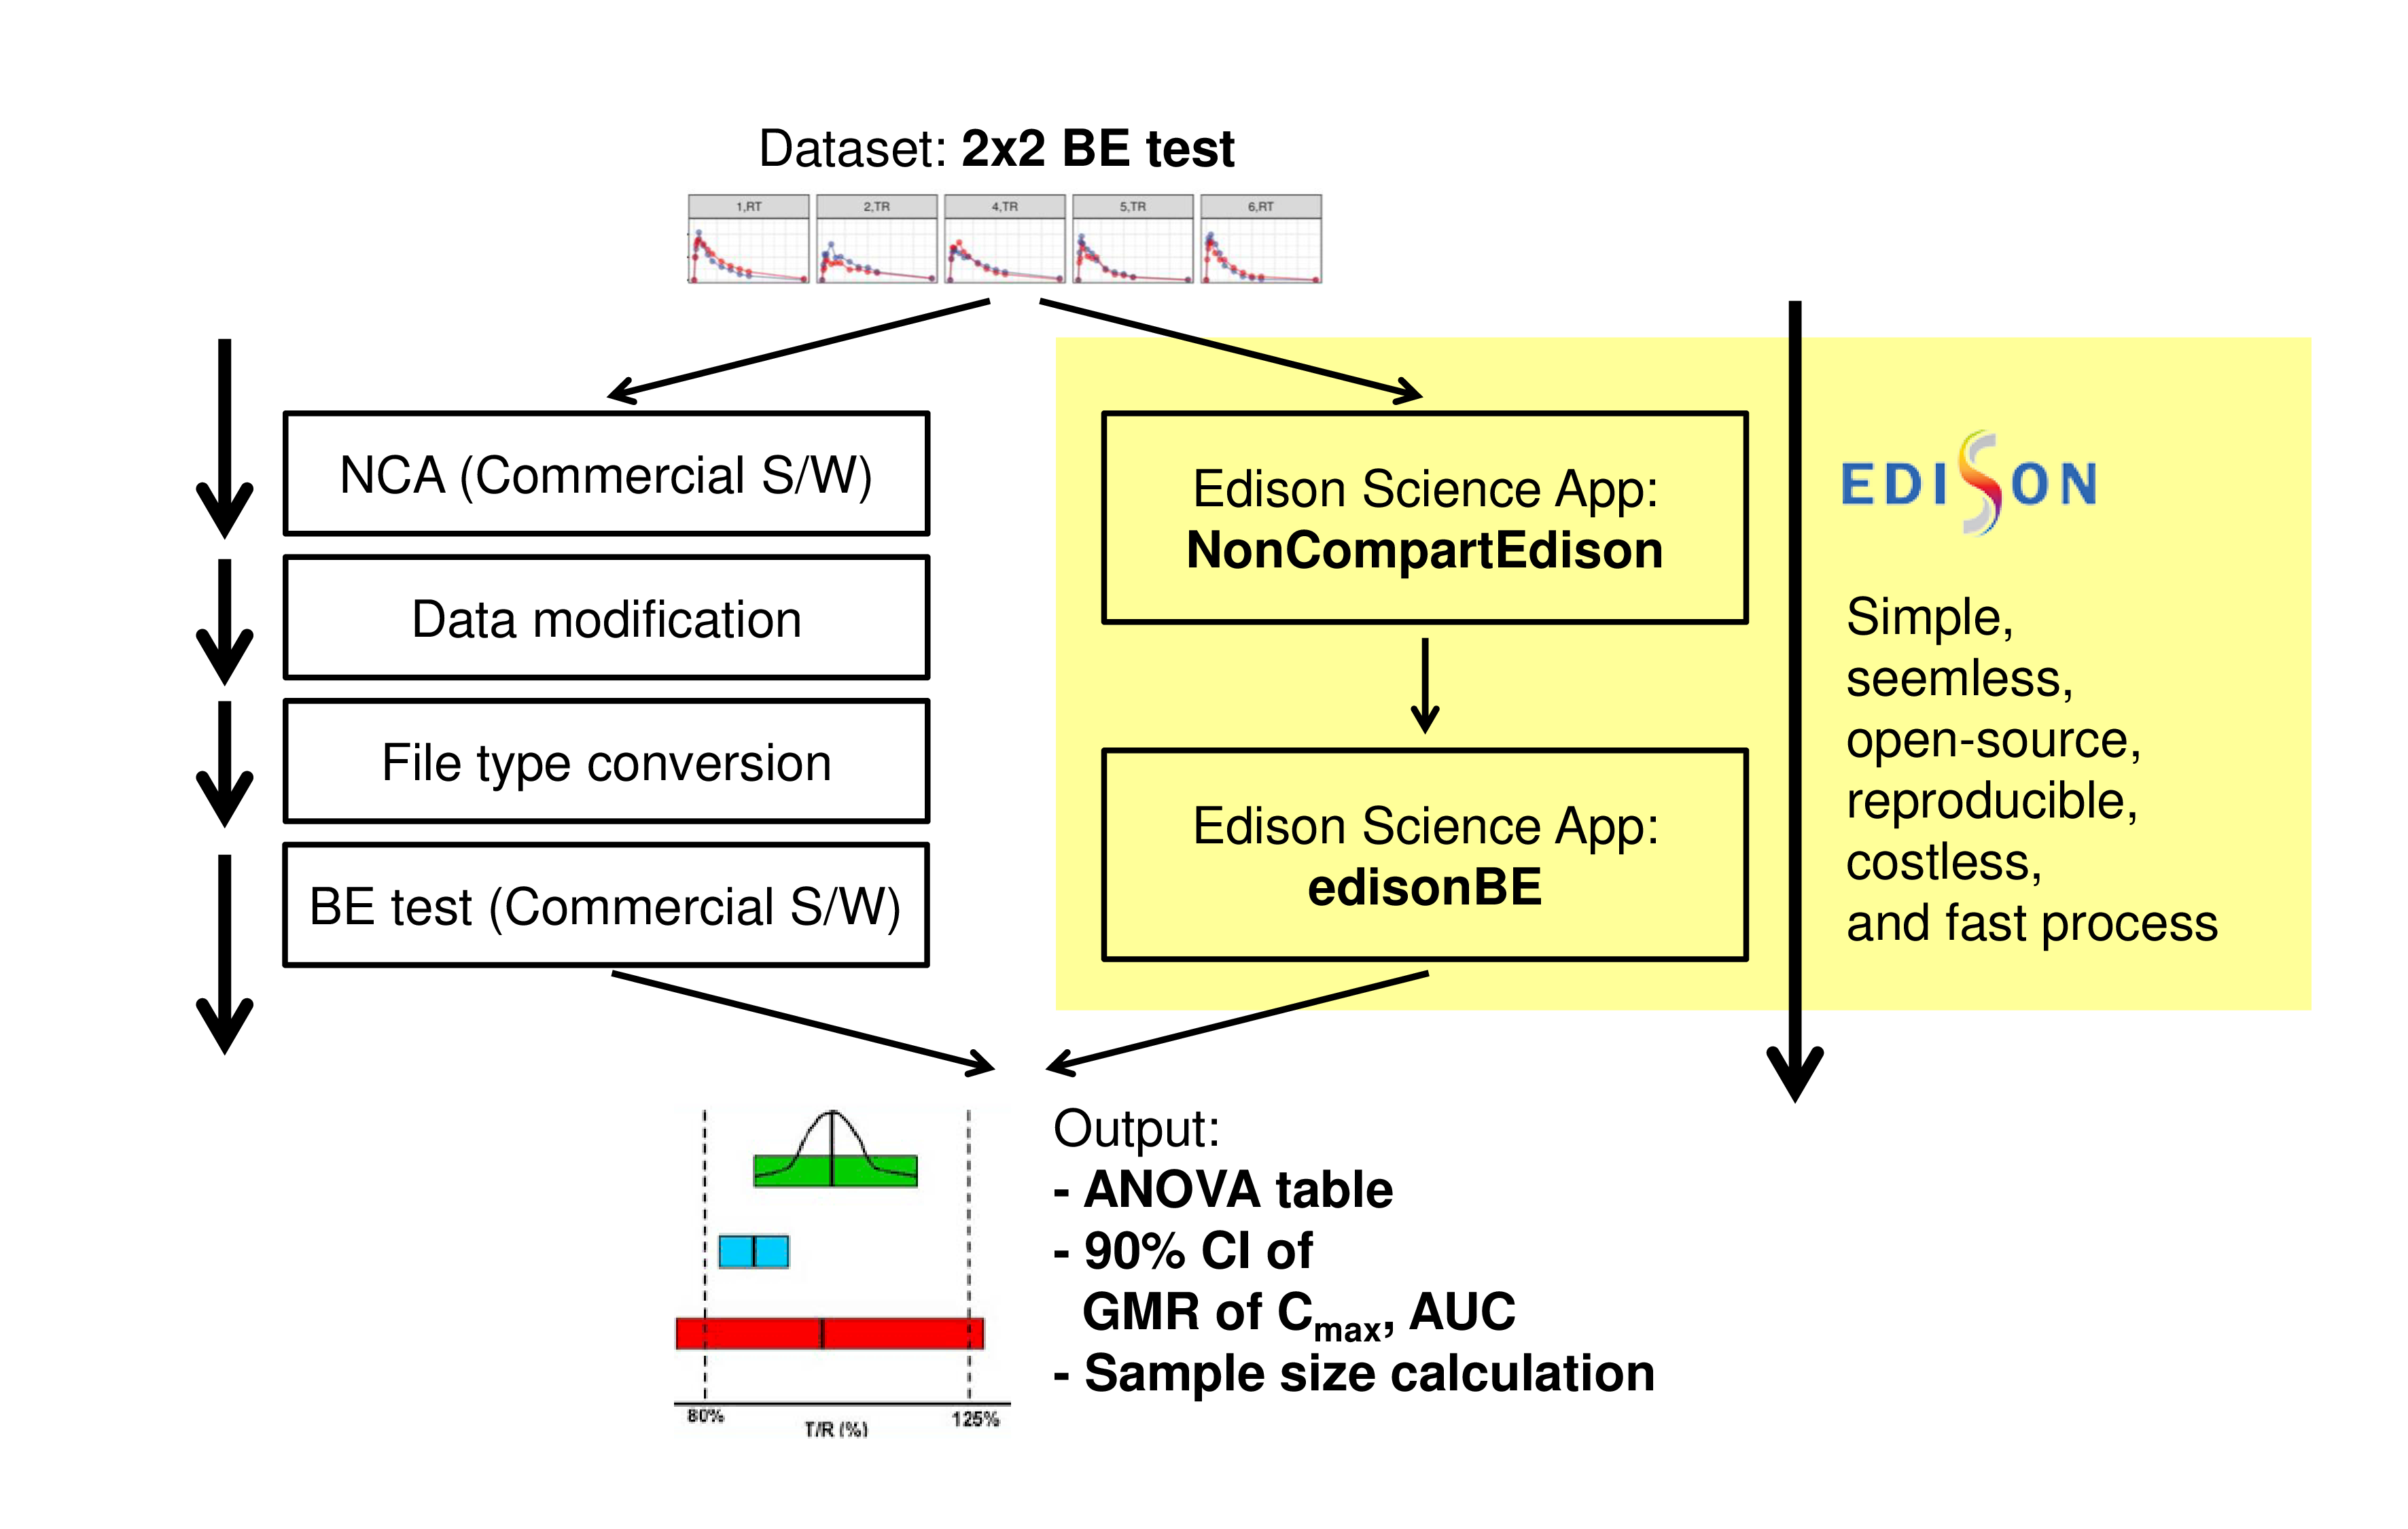
\includegraphics{assets-paper/figure-3.png}

Figure 3. Comparison between a traditional analysis process (left boxes) and the proposed process (right boxes) using EDISON Science Apps.

본 연구는 EDISON 사이언스 앱을 사용해 쉽고 정확하고 비용이 들지 않는 빠른 비구획분석과 생물학적동등성 분석법을 제시하였다.
현재는 이러한 분석을 위해서 여러 상용 소프트웨어를 필요로 하는 복잡한 단계를 거쳐야 한다. (Figure 3) 따라서 분석 시간이 오래 걸리고 많은 비용이 소모되었다. 본 저자들은 EDISON 사이언스 앱을 사용하여 이 두 과정을 통합하였고, 이로서 농도-시간 자료로부터 비구획분석과 생물학적동등성 통계 분석까지 연속적으로 가능케 하였다.
본 분석에서 학계와 산업계에서 가장 정확하게 생물학적 동등성을 평가한다고 말하는 SAS통계 패키지와의 비교를 통해 EDISON 사이언스 앱을 사용한 생물학적 동등성 분석이 정확한 값을 제시함을 검증할 수 있었다.
학생들의 교육에 효과적인 EDISON 사이언스 앱으로 개발되어 약리학 과목의 필수항목인 약동학의 교육에의 활용도 기대된다. 또한 임상시험 산업계에서도 많은 비용을 절감할 수 있을 것으로 기대된다.
아직은 2x2 교차 설계에서 얻어진 자료로만 분석이 가능하다는 한계를 갖고 있지만 앞으로 다양한 설계를 갖는 자료가 사용 가능하도록 업데이트가 가능할 것이다.

\hypertarget{conclusion}{%
\chapter{결론}\label{conclusion}}

본 연구가 제시하는 EDISON 사이언스 앱을 통한 방법을 통해 정확한 분석을 빠른 시간에 수행할 수 있을 뿐만 아니라 오류를 줄이고 비용을 절감하는 효과를 가져올 수 있다.

\hypertarget{acknowledgement}{%
\chapter{감사의 글}\label{acknowledgement}}

본 논문은 정부(과학기술정보통신부)의 재원으로 한국연구재단 첨단 사이언스·교육 허브 개발 사업의 지원을 받아 수행된 연구임(NRF-2011-0020576)

\hypertarget{references}{%
\chapter{참고문헌}\label{references}}

\begin{enumerate}
\def\labelenumi{\arabic{enumi}.}
\tightlist
\item
  식품의약품안전청 식. 동등생물의약품 평가 가이드라인. 2009.
\item
  Chow S-C, Liu J-p.~Design and analysis of bioavailability and bioequivalence studies. Chapman \& Hall/CRC biostatistics series, vol 27, 3rd edn. CRC Press, Boca Raton, 2009
\item
  Yoon S-H, Hwang N-A, Lim Y-C, Lee Y-B, Park J-S. Development of BioEquiv, a Computer Program for the Analysis of Bioequivalence. Journal of Korean Pharmaceutical Sciences 2010;40:1-7. doi: 10.4333/kps.2010.40.1.001.
\item
  R Core Team, R Foundation for Statistical Computing. R: A Language and Environment for Statistical Computing. \url{https://www.R-project.org/} 2018
\end{enumerate}


\end{document}
